\documentclass{beamer}

\usepackage[utf8]{inputenc}
\usepackage{listings}

\usepackage{xcolor}
\usetheme{AnnArbor}
\useinnertheme{rectangles}
\usecolortheme{crane}

\beamertemplatenavigationsymbolsempty

\AtBeginSection[] {
	\begin{frame}<beamer>
		\frametitle{Overview}
		\tableofcontents[currentsection]
	\end{frame}
}

\begin{document}
\title{Group-OTR library}
\subtitle{Peer-to-Peer Systems and Security}
\author{
	Markus Teich
	\and
	Jannik Theiß
}
\date{\today}

\frame{\titlepage}

\frame{
	\frametitle{Overview}
	\tableofcontents
}

\section{Motivation}

\frame{
	\frametitle{Motivation}
	secure online conversations for everyone\vfill \pause
	significance of social communication via internet for society
}


\frame{
	\frametitle{Everyone?}
	\begin{itemize}
		\item{people who are no computer scientists}\pause
		\item{people who have no higher education\\ \pause
		$\Rightarrow$ must be easy to use\pause}
		\item{people who are not motivated to use secure communication\\ \pause
		$\Rightarrow$ should be default}
	\end{itemize}
}

\frame{
	\frametitle{Problem with new solutions}
	\begin{itemize}
		\item{hard to motivate users to switch platforms \pause}
		\item{hard to predict what the next popular platform will be\\ \pause
		$\Rightarrow$ native as well as plugin intergration\pause}
	\end{itemize}
	\center
	\vfill
	$\Rightarrow$ independent library
}

\frame{
	\frametitle{goal of (group) OTR}
	provide properties of personal face to face conversations\pause
	\begin{itemize}
		\item{recognition of other participants\pause}
		\item{only participants know what was said\pause}
		\item{everyone hears the same\pause}
		\item{honest word is the only proof to third parties}
	\end{itemize}
}

\frame{
	\frametitle{technical goals}
	\begin{itemize}
		\item{entity authenticity\pause}
		\item{origin authenticity\pause}
		\item{integrity\pause}
		\item{confidentiality\pause}
		\item{forward secrecy\pause}
		\item{deniability\pause}
		\item{transcript consistency}
	\end{itemize}
}

\frame{
	\frametitle{our library}
	\begin{itemize}
		\item{synchronous multi party communication\pause}
		\item{easy to use/integrate\pause}
		\item{minimal dependencies\pause}
		\item{suitable for peer-to-peer\pause}
		\item{open source + free to use}
	\end{itemize}
}

\section{Related work}

\frame{
	\frametitle{OTR (Borisov, Goldberg and Brewer \cite{otr})}
	\begin{itemize}
		\item{synchronous}
		\item{2-party\pause}
		\item{forward secrecy: consecutive Diffie–Hellman key exchanges\pause}
		\item{deniability: shared MAC keys}
	\end{itemize}
}

\frame{
	\frametitle{Improved User Authentication in OTR (Alexander and Goldberg \cite{auth-otr})}
	\center
	how to get the public key?\\ \pause
	$\Rightarrow$ socialist millionaire protocol
}

\frame{
	\frametitle{OTR for groups (Bian, Seker, Topaloglu \cite{gotr})}
	\begin{itemize}
		\item{uses standard 2-party OTR\pause}
		\item{chooses one node as virtual server\pause}
		\item{virtual server has to be trusted}
	\end{itemize}
}

\frame{
	\frametitle{TextSecure \cite{textsecure-group}}
	\begin{itemize}
		\item{asynchronous\pause}
		\item{server based\pause}
		\item{uses individual direct connections for group conversations\pause}
		\item{transcript is not (yet) consistency-checked}
	\end{itemize}
}

\frame{
	\frametitle{mpOTR (Goldberg, Ustaoğlu, Van Gundy, Chen \cite{mp-otr})}
	\begin{itemize}
		\item{new OTR-like protocol for group conversations\pause}
		\item{consistency surprise}
	\end{itemize}
}

\frame{
	\frametitle{GOTR (Liu, Vasserman, Hopper \cite{impr-gotr})}
	\center
	solves several problems of mpOTR, including consistency surprise
}


\section{GOTR}

\frame{
	\frametitle{Burmester-Desmedt GKA}
	Nodes $D = \{D_1, ..., D_n\}$\\ \pause
	$\forall D_l \in D:$
	\begin{enumerate}
		\item{generate private key $r_l$\pause}
		\item{$z_l = g^{r_l} \mod p$\pause}
		\item{send $z_l$ to neighbours\pause}
		\item{$X_l = (z_{l+1} / z_{l-1})^{r_l} \mod p$\pause}
		\item{broadcast $X_l$\pause}
		\item{$\kappa = (z_{l-1})^{n r_l} * X^{n-1}_{l} * X^{n-2}_{l+1} * ... * X_{l-2} \mod p$\\ \pause
		$= g^{r_1*r_2 + r_2*r_3 + ... + r_n*r_1}$}
	\end{enumerate}
}

\frame{
	\frametitle{GOTR}
	\begin{itemize}
		\item{Setup\pause}
		\item{KeyUpdate\pause}
		\item{Communicate: SendMsg, RecvMsg, ConsCheck}
	\end{itemize}
}

\frame{
	\frametitle{GOTR: Setup}
	\begin{itemize}
		\item{performed by a joining participant\pause}
		\item{establish private channel to each other participant}
		\begin{itemize}
			\item{authenticated}
			\item{confidential}
			\item{don't have to be deniable or forward-secret\pause}
		\end{itemize}
		\item{obtain cryptographic digest}
	\end{itemize}
}

\frame{
	\frametitle{GOTR: KeyUpdate}
	\begin{itemize}
		\item{generate fresh keys used for encryption and authentication\pause}
		\item{every $D_i$ acts as two nodes per other participant\pause}
		\item{every $D_i$ generates his cycle-key $K_i$\pause}
		\item{derive $k_{i1}$ and $k_{i2}$ from $K_i$}
	\end{itemize}
}

\frame{
	\frametitle{GOTR: Cycle-key generation}
	\center
	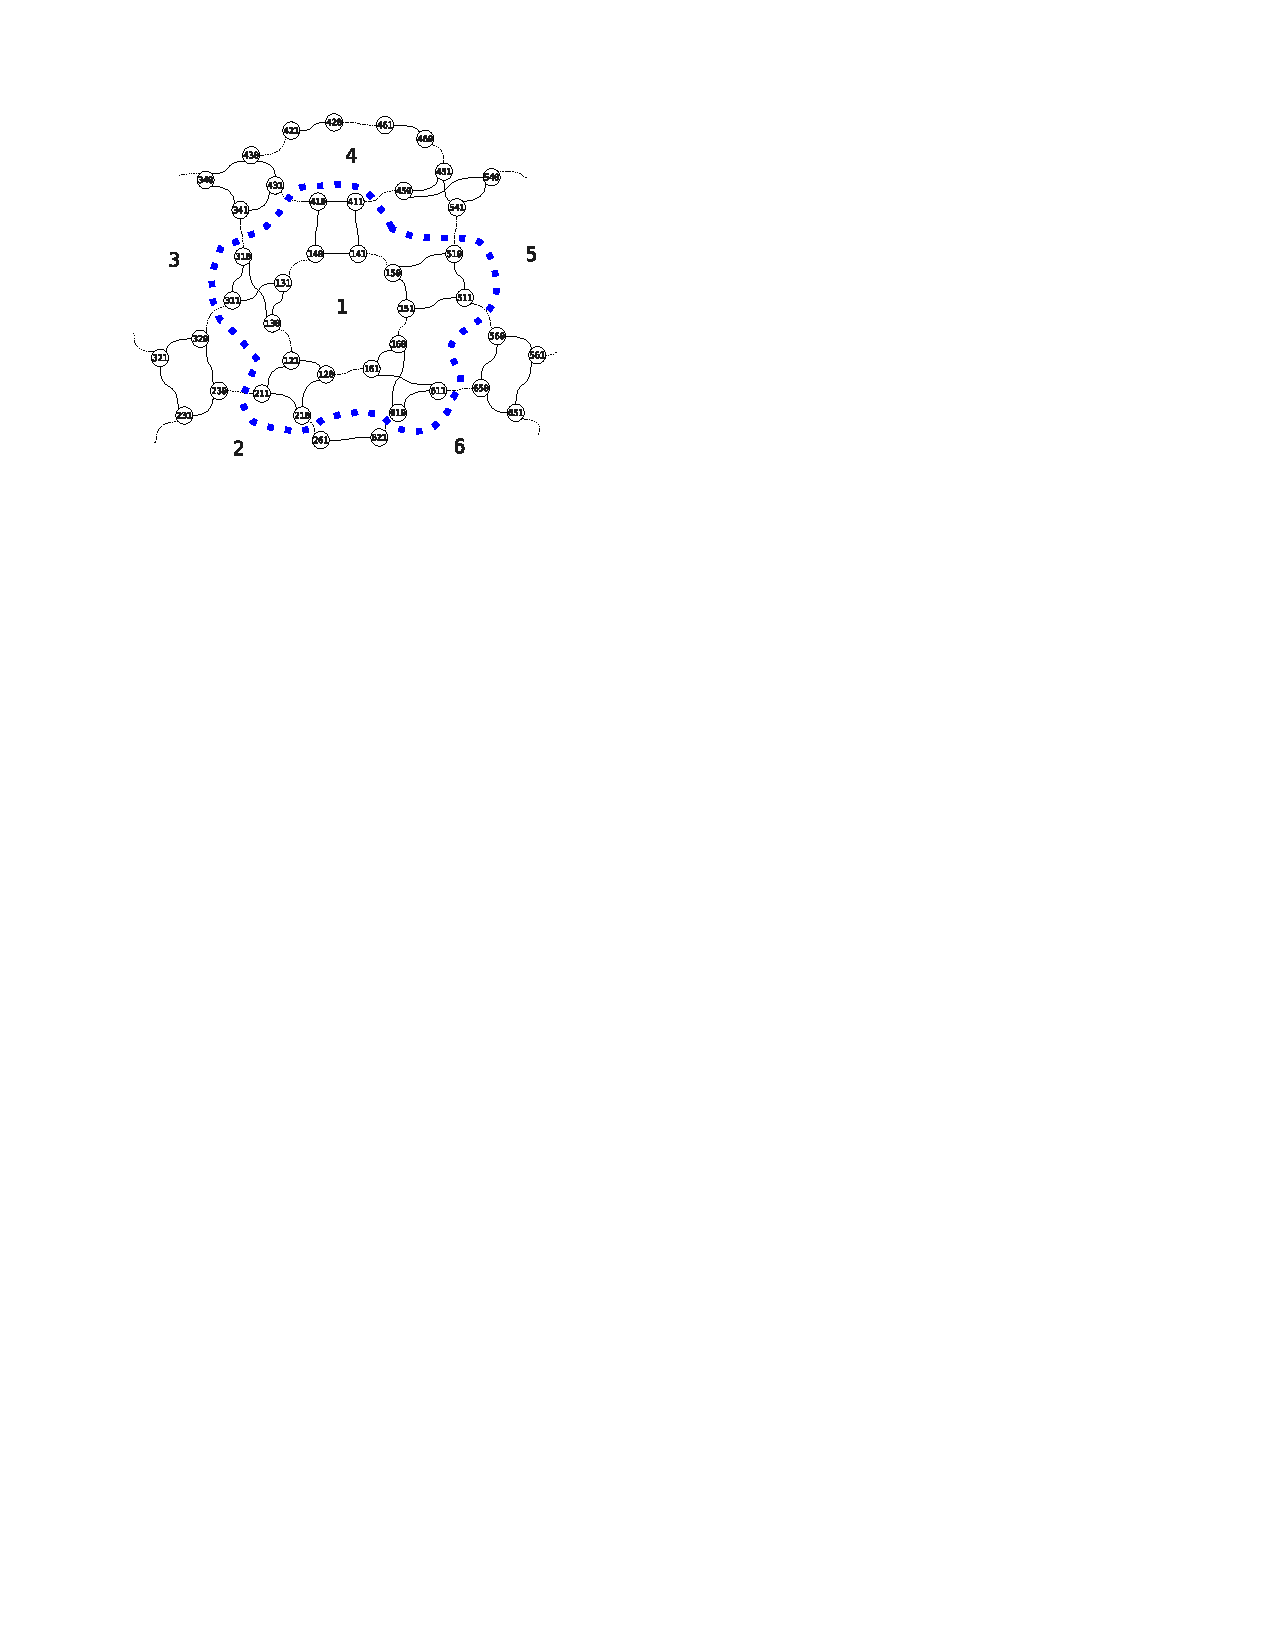
\includegraphics[width=250px]{cycle-keys.pdf}
}

\frame{
	\frametitle{GOTR: Communication}
	\begin{itemize}
		\item{SendMsg}
		\begin{itemize}
			\item{encrypted and authenticated with $k_{i1}$ and $k_{i2}$\pause}
			\item{piggyback $z$-$X$-pairs values and digest\pause}
		\end{itemize}
		\item{RecvMsg}
		\begin{itemize}
			\item{match $z$-$X$-pairs with previously received ones to determine author\pause}
		\end{itemize}
		\item{ConsCheck}
		\begin{itemize}
			\item{exchange digest with every other user over the private channels}
		\end{itemize}
	\end{itemize}
}

\section{libgotr}

\frame{
	\frametitle{libgotr}
	\begin{itemize}
		\item{based on libgcrypt (Curve25519, EdDSA, ECDHE, AES/twofish)}
	\end{itemize}
}

\frame{
	\frametitle{libgotr API}
	\lstinputlisting[]{api2.c}
}

\frame{
	\frametitle{libgotr API}
	\lstinputlisting[]{api3.c}
}

\frame{
	\center
	Thank you for your attention!
}

\frame[allowframebreaks]{
\frametitle{References}
\begin{thebibliography}{xx}

	\bibitem{otr} N. Borisov, I. Goldberg, and E. Brewer. Off-the-record
		communication, or, why not to use PGP. In \textit{Proceedings of the ACM
		workshop on Privacy in the electronic society}, WPES ’04, 2004.

	\bibitem{sec-otr} M. Di Raimondo, R. Gennaro, and H. Krawczyk. Secure
		off-the-record messaging. In \textit{Proceedings of the ACM workshop on
		Privacy in the electronic society}, WPES ’05, 2005.

	\bibitem{auth-otr} C. Alexander and I. Goldberg. Improved User
		Authentication in Off-the-Record Messaging. In \textit{Proceedings of
		the 2007 ACM workshop on Privacy in electronic society}, WPES ’07, 2007.

	\bibitem{gotr} J. Bian, R. Seker, and U. Topaloglu. Off-the-Record Instant
		Messaging for Group Conversation. In \textit{Proceedings of Information
		Reuse and Integration}, IRI ’07, 2007.

	\bibitem{user-study} R. Stedman, K. Yoshida, and I. Goldberg. A User Study
		of Off-the-Record Messaging. In \textit{Proceedings of the Symposium On
		Usable Privacy and Security}, SOUPS ’07, 2008.

	\bibitem{mp-otr} I. Goldberg, B. Ustaoğlu, M. D. Van Gundy, and H. Chen.
		Multi-party Off-the-Record Messaging. In \textit{Proceedings of the ACM
		Conference on Computer and communications security}, CCS ’09, 2009.

	\bibitem{impr-gotr} H. Liu, E. Y. Vasserman, and N. Hopper. Improved Group
		Off-the-Record Messaging. In \textit{Proceedings of the ACM workshop on
		Privacy in the electronic society}, WPES ’11, 2013.
	
	\bibitem{textsecure-group} Textsecure: Private Group Messaging \textit{https://whispersystems.org/blog/private-groups/}.

\end{thebibliography}
}

\end{document}
